\subsection{过滤器模式(Filter)}

过滤器模式(Filter Pattern)或标准模式(Criteria Pattern)是一种设计模式,这种模式允许开发人员使用不同的标准来过滤一组对象,通过逻辑运算以解耦的方式把它们连接起来。这种类型的设计模式属于结构型模式,它结合多个标准来获得单一标准。

\begin{figure}[h]
  \centering
  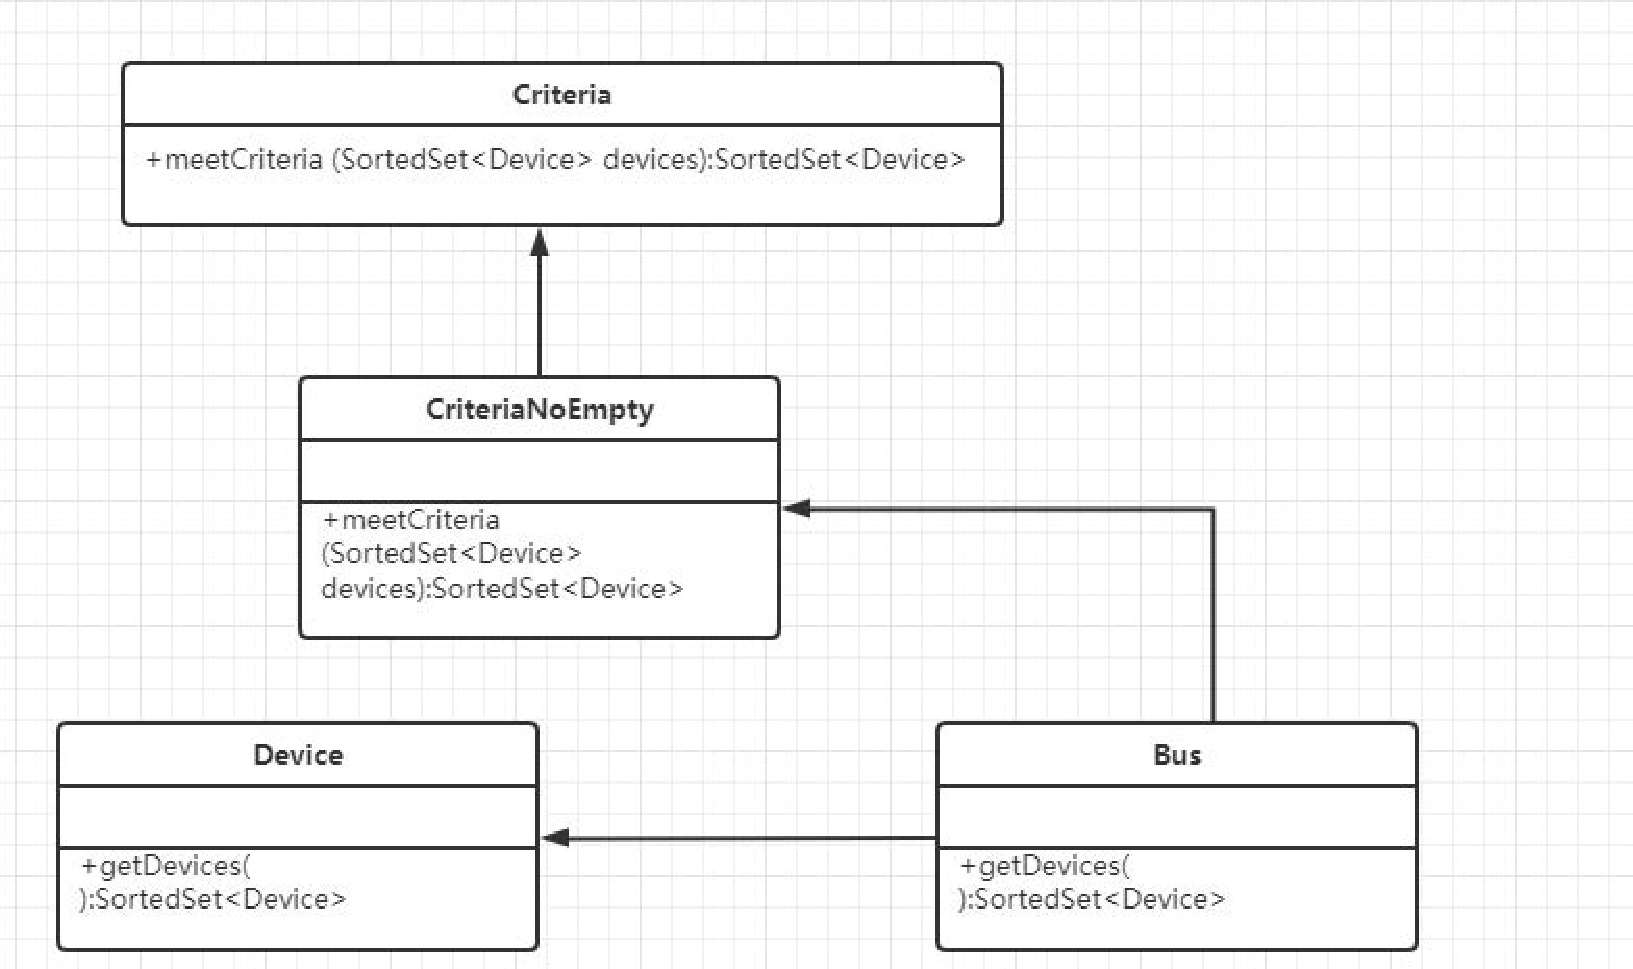
\includegraphics[width=0.9\textwidth]{figures/过滤器模式.pdf}
  \caption{过滤器模式在 Slow6502 中的类图}
\end{figure}

使用过滤器可以有效地提高模拟器的性能。在模拟器中,通常需要处理大量的数据,并且这些数据可能非常复杂。如果模拟器的代码不进行优化,就可能会导致性能下降,影响模拟器的效率。使用过滤器可以提高模拟器的性能,因为它可以帮助模拟器更快地处理数据。过滤器可以将大量的数据缩小到更小的范围,使模拟器只需处理有用的数据,而不是所有的数据。这样做可以让模拟器更快地运行,提高效率。此外,使用过滤器还可以让模拟器的代码更容易理解和维护。过滤器可以把复杂的数据处理过程分解成一系列简单的步骤,使代码更加清晰易懂。这样,程序员可以更容易地查看和修改代码,避免出现错误。

总的来说,使用过滤器可以提高模拟器的性能,让代码更容易理解和维护。

